% Template for Cogsci submission with R Markdown

% Stuff changed from original Markdown PLOS Template
\documentclass[10pt, letterpaper]{article}

\usepackage{cogsci}
\usepackage{pslatex}
\usepackage{float}
\usepackage{caption}

% amsmath package, useful for mathematical formulas
\usepackage{amsmath}

% amssymb package, useful for mathematical symbols
\usepackage{amssymb}

% hyperref package, useful for hyperlinks
\usepackage{hyperref}

% graphicx package, useful for including eps and pdf graphics
% include graphics with the command \includegraphics
\usepackage{graphicx}

% Sweave(-like)
\usepackage{fancyvrb}
\DefineVerbatimEnvironment{Sinput}{Verbatim}{fontshape=sl}
\DefineVerbatimEnvironment{Soutput}{Verbatim}{}
\DefineVerbatimEnvironment{Scode}{Verbatim}{fontshape=sl}
\newenvironment{Schunk}{}{}
\DefineVerbatimEnvironment{Code}{Verbatim}{}
\DefineVerbatimEnvironment{CodeInput}{Verbatim}{fontshape=sl}
\DefineVerbatimEnvironment{CodeOutput}{Verbatim}{}
\newenvironment{CodeChunk}{}{}

% cite package, to clean up citations in the main text. Do not remove.
\usepackage{apacite}

% KM added 1/4/18 to allow control of blind submission
\cogscifinalcopy

\usepackage{color}

% Use doublespacing - comment out for single spacing
%\usepackage{setspace}
%\doublespacing


% % Text layout
% \topmargin 0.0cm
% \oddsidemargin 0.5cm
% \evensidemargin 0.5cm
% \textwidth 16cm
% \textheight 21cm

\title{Cognitive diversity in context: US-China differences in
children's reasoning, visual attention, and social cognition}


\author{Alexandra Carstensen$^{1}$ (abcarstensen@asu.edu), Anjie Cao$^{2}$  (anjiecao@stanford.edu), \\ \bf{Alvin W. M. Tan$^2$ (tanawm@stanford.edu)}, \bf{Di Liu$^3$ (dliu88@jh.edu)}, \bf{Yichun Liu$^4$ (18307110502@fudan.edu.cn)}, \\ \bf{Minh K. Bui$^5$ (mbui100@csu.fullerton.edu)}, \bf{Jiayi Wang-Zhao$^6$ (jiayiwang@fas.harvard.edu)}, \\ \bf{Ai Nghi Diep$^2$ (ainghi@stanford.edu)}, \bf{Qi Han$^2$ (qihan96@stanford.edu)}, \\ \bf{Michael C. Frank$^2$ (mcfrank@stanford.edu)}, and \bf{Caren M. Walker$^7$ (carenwalker@ucsd.edu)} \\ $^1$Psychology, School of Social and Behavioral Sciences, Arizona State University, $^2$Psychology, Stanford University, \\ $^3$Psychological and Brain Sciences, Johns Hopkins University,  $^4$Psychology, Fudan University, \\ $^5$Communication Sciences, CSU Fullerton,  $^6$Psychology, Harvard University,  $^7$Psychology, UC San Diego}

\newlength{\cslhangindent}
\setlength{\cslhangindent}{1.5em}
\newenvironment{CSLReferences}%
  {}%
  {\par}

\begin{document}

\maketitle

\begin{abstract}
Outward differences between cultures are very salient, with Western and
East Asian cultures as a prominent comparison pair. A large literature
describes cross-cultural variation in cognition, but relatively less
research has explored the developmental origins of this variation. This
study helps to fill the empirical gap by replicating four prominent
findings documenting cross-cultural differences in children's reasoning,
visual attention, and social cognition in a cross-sectional sample of
240 3-12-year-olds from the US and China. We observe cross-cultural
differences in three of the four tasks and describe the distinct
developmental trajectory that each task follows throughout early and
middle childhood.

\textbf{Keywords:}
cognitive development; culture; variation; reasoning; attention; social
cognition; US; China; replication.
\end{abstract}

\hypertarget{introduction}{%
\section{Introduction}\label{introduction}}

Learning and cognitive development are embedded in and shaped by
cultural variation; children show sensitivity to and specialization for
their unique perceptual environment before birth, discriminating
familiar voices and languages (DeCasper \& Fifer, 1980; Moon, Cooper, \&
Fifer, 1993), and imitating the intonation of familiar languages within
their first week (Mampe, Friederici, Christophe, \& Wermke, 2009).
Variation across cultures continues to play an important role in
cognition over the lifespan, and while the literature documenting
cross-cultural variation is extensive, much of this work is focused on
differences between adults. How and when do these specific differences
arise?

Perhaps the best developed empirical foundation for examining these
questions is the contrast between Western and East Asian cultures,
particularly the United States and China, which have become focal points
for cultural difference comparisons (Muthukrishna et al., 2020).
Previous research has described differences between US and Chinese
populations in self-concepts (Boucher, 2011; Spencer-Rodgers, Boucher,
Mori, Wang, \& Peng, 2009), values (Ji, Nisbett, \& Su, 2001; Kwan,
Bond, \& Singelis, 1997; Spencer-Rodgers, Williams, Hamilton, Peng, \&
Wang, 2007), preferences (Corriveau et al., 2017; DiYanni, Corriveau,
Kurkul, Nasrini, \& Nini, 2015; Liang \& He, 2012), social cognition
(Morris \& Peng, 1994), similarity judgments (Ji, Zhang, \& Nisbett,
2004), relational reasoning (Carstensen et al., 2019; Cheng, 2020;
Richland, Chan, Morrison, \& Au, 2010), language learning (Chan et al.,
2011; Tardif, 1996; Waxman et al., 2016), executive function (Sabbagh,
Xu, Carlson, Moses, \& Lee, 2006; Tan, 2020), and visual attention
(Chua, Boland, \& Nisbett, 2005; Ji, Peng, \& Nisbett, 2000; Waxman et
al., 2016), among others.

Given the breadth, depth, and sheer volume of this research, it is
difficult to synthesize the findings to understand the locus of causal
mechanisms, the relationships between behavior in various tasks, and the
sources of differences. For instance, while cultures are often viewed as
collectivistic and individualistic to varying degrees, measurement of
these constructs with individual people (the typical unit of measurement
in cross-cultural comparisons) has proven problematic and often
unreliable (e.g., Oyserman, Coon, \& Kemmelmeier, 2002; Takemura, Yuki,
Maddux, \& Ohtsubo, 2007; for a review see Wong, Wang, \& Klann, 2018),
leading to the formulation of related but alternative cultural
constructs at the level of individuals, like interdependent and
independent self-construal (Markus \& Kitayama, 1991; Singelis, 1994),
and holistic and analytic processing (Koo, Choi, \& Choi, 2018; Peng \&
Nisbett, 1999). However, across 10 measures of independent and
interdependent social orientation and 10 of analytic and holistic
cognitive style, Na et al. (2010) found little evidence that consistent
individual differences underlie group-level cultural differences,
complicating psychological explanations that link social organization to
human cognition. One of the key challenges in this literature is that of
mapping from country-level cultural constructs like collectivism to
individual-level behavior measured in psychological tasks.

Several proposals (e.g., Markus \& Kitayama, 2010; Miyamoto, 2013)
address the complexities of mapping between abstract cultural features
(e.g., Confucian-heritage philosophy) and individual behavior (e.g.,
tendency towards holistic processing). Miyamoto (2013) argues for
multilevel analyses that bridge from the distal, societal factors most
prominently discussed in the cultural psychology literature, to proximal
situational processes (e.g., childhood experiences) that motivate
differences in cognition. For example, the focused attention exemplified
in American mothers' child-directed speech might socialize children
toward more analytic processing styles, compared to the more dynamic,
relational play of Japanese mothers, which may scaffold toward more
holistic cognitive processing. Because many cross-cultural differences
emerge by the time that adults are college-aged, these proximal contexts
are necessarily developmental contexts: they are the contact points
between culturally specific experience (like growing up in a
Confucian-heritage culture) and the cognitive differences that result
from this variation (like a tendency toward holistic processing).
Unfortunately, proximal contexts like these are not yet well documented.

We see a fundamental part of this puzzle as developmental: what
cognitive mechanisms underlie behavioral differences, and what are the
intermediate, proximal contexts in which children receive information
about distal societal factors? When do various cross-cultural
differences begin to appear, and what is the developmental trajectory to
adulthood? As an initial step toward identifying these culture-specific
learning environments and the processing mechanisms they support,
research is needed to document the initial appearance of these
differences, and their developmental progression.

\hypertarget{the-present-study}{%
\subsection{The present study}\label{the-present-study}}

In this work, we aim to replicate previously attested differences
between children in the US and China and to measure the developmental
trajectories of these differences. We build conceptually on work by
Carstensen et al. (2019) showing that young children (1.5 -- 4.0 years)
in the US and China follow unique developmental trajectories in
relational reasoning. Our cross-sectional sample begins where this prior
work left off, examining relational reasoning alongside visual attention
and social reasoning tasks, which have been shown to differ across
cultures in prior work.

We considered three main desiderata in our task selection: tasks must be
short, appropriate for administration across a large range of ages, and
theoretically implicated in relational reasoning (for a review of
accounts linking relational reasoning to other cross-cultural
differences, see Christie, Gao, \& Ma, 2020). We included measures of
social reasoning and visual attention, building directly on the methods
of a prior study with adults (Cao and Carstensen et al., in press). This
prior work explored the robustness of attested cross-cultural
differences across 12 experimental paradigms for adults, only 5 of which
yielded robust differences in the predicted direction. This degree of
reproducibility is consistent with large-scale reproducibility studies
within psychology (Collaboration, 2015), but issues limiting
replicability may well be more severe in developmental research, where
they are much less explored (Frank et al., 2017; Gennetian, Frank, \&
Tamis-LeMonda, 2022). In summary, the present work serves two purposes:
it is intended as one step of many toward a more robust developmental
science, and as an initial step toward cognitive characterization of
cross-cultural differences.

\hypertarget{methods}{%
\section{Methods}\label{methods}}

\hypertarget{participants}{%
\subsection{Participants}\label{participants}}

We recruited a cross-sectional sample of children between 3 and 12 years
old through snowball sampling of parents seeded at large universities in
the US and China. Researchers directly recruited some participants and
those participants recruited others through referrals, social media
sharing, and email forwarding at the researchers' request. Additional
recruitment was conducted through lab databases (for US participants),
social media posts (CN participants), and elementary schools (CN).
Parents received a certificate of completion as a thank-you for
participating in the study, and those recruited through databases that
use parental compensation received a \$5 gift card. We recruited 240
children, 120 per country in the US and China, sampling 40 participants
in each of three age ranges (3-6, 7-9, and 10-12 years old) from each
cultural context.

After exclusions, the US sample included 108 children (54 male, 54
female), all native speakers of English. The China sample included 117
children (75 male, 41 female, 1 declined to answer), all native speakers
of Mandarin Chinese. Additionally, we excluded participants from the
analysis of individual tasks if they were missing more than 25\% of the
data from that task, failed to follow instructions, or showed a side
bias (choosing the left or right option on all four trials of the
relational reasoning task).

\hypertarget{procedure}{%
\subsection{Procedure}\label{procedure}}

Participants were presented with a set of four tasks measuring
relational reasoning, social reasoning, and visual attention, and their
parents completed a family demographics questionnaire. An experimenter
guided each child through the experiment via video call, with stimuli
presented through a shared webpage. The experiment was administered in
English for participants in the US, and in Mandarin Chinese for those in
China, with both written and spoken instructions to minimize the effect
of varied reading ability across children. Tasks were presented in a
randomized order, with the exception of the Uniqueness Preference task.
This task was always presented last to support the task cover story,
which congratulated the child for nearing the end of the session. The
experiment took about 20 minutes to complete.

\hypertarget{tasks}{%
\subsection{Tasks}\label{tasks}}

\hypertarget{relational-preference-crmts}{%
\subsubsection{Relational Preference
(cRMTS)}\label{relational-preference-crmts}}

Carstensen et al. (2019) describe distinct developmental trajectories
for relational reasoning performance in the US and China that correspond
to different biases toward object-based and relational solutions. They
measured relational and object bias in a causal relational
match-to-sample (cRMTS) task, finding that 3-year-olds from the US
preferred object-based solutions (e.g., blue cubes activate a machine)
while those from China preferred relational solutions (e.g., pairs of
different objects activate a machine). We use the same ambiguous cRMTS
task, presenting evidence consistent with both object and relational
solutions, to measure children's bias from age 3 to 12 in both cultures.
Our participants were shown two pairs of blocks exemplifying the
different relation (schematically, AB and AC) that made a machine play
music. They could then chose between an object-based solution (same pair
AA) and a relational solution (different pair BC) to activate the
machine in the test phase (see the procedure schematic in Figure 1. On
the first test trial, the two choices recombined blocks presented during
training into novel pairs composed of familiar blocks (AA vs.~BC). We
added three additional trials that each present a choice between the
object-based solution (same pair AA) and novel relational solutions
(different pairs DE, FG, HI), to provide multiple trials with each
participant without exactly repeating the answer choices from the first
trial.\footnote{NB: the first trial is truly ambiguous, forcing a choice between blocks that were all associated with machine activation during training but implement different relations, while the logic of the later trials necessarily relies on generalization from different pairs composed of novel instead of familiar blocks. This design is necessary to create additional test trials with block pairs distinct from the first trial.}

\begin{CodeChunk}
\begin{figure}[H]

{\centering 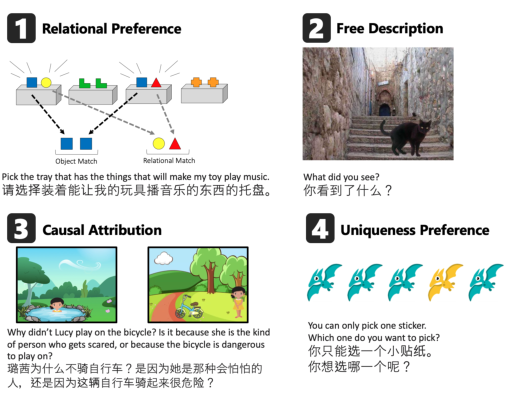
\includegraphics{figs/image-1} 

}

\caption[Methods overview for the tasks measuring relational reasoning (1), visual attention (2), and social reasoning (3 and 4)]{Methods overview for the tasks measuring relational reasoning (1), visual attention (2), and social reasoning (3 and 4).}\label{fig:image}
\end{figure}
\end{CodeChunk}

\hypertarget{picture-free-description}{%
\subsubsection{Picture Free
Description}\label{picture-free-description}}

In a classic study, Masuda \& Nisbett (2001) showed that adults in the
US and Japan focus on different elements of scenes when describing them
from memory, with Japanese adults providing more information about the
scene context and background, particularly at the beginning of their
description. Imada, Carlson, \& Itakura (2013) found similar differences
between children: Japanese children provided more description of scene
backgrounds and tended to describe peripheral and background elements of
scenes first, while their US counterparts were more likely to mention
the focal object first. Cao and Carstensen et al. (in press) extended
this work, documenting similar differences between adults in the US and
China. Following Cao and Carstensen et al. (in press), we showed our
participants seven images from the Imada et al. (2013) study, each for
15 seconds, and then asked them to describe what they saw, prompting for
additional information up to three times (e.g., ``Anything else?'', ``Is
that all?'') and moving on after the third prompt or when the child
agreed their description was complete. We coded the first item mentioned
in each description (focal or background) and completed a detailed
coding of the full description following the original Michigan Fish Task
protocol (Masuda \& Nisbett, 2001).

\hypertarget{causal-attribution}{%
\subsubsection{Causal Attribution}\label{causal-attribution}}

East Asians are more likely than people from Western countries to make
attributions about behavior that reference specifics of a particular
situation, compared with dispositions of a particular person (Morris \&
Peng, 1994; for replication, see Cao and Carstensen et al., in press).
For example, Seiver, Gopnik, \& Goodman (2013) found that when children
were asked to explain why two children engaged in one activity and
avoided another (highlighting situational constraints), 6-year-old
children from the US were equally likely to make personal and
situational attributions, neglecting the evidence in favor of
situational causes. We replicated this work, which showed a series of
four short vignettes to participants. In these vignettes, two children
both jumped into a pool, while neither of them played on a bicycle. We
asked participants to explain why each child in the vignette refused to
play with the bicycle, explicitly prompting for personal or situational
attributions (e.g., ``Why didn't Kelly play on the bicycle? Is it
because she is the kind of person who gets scared, or because the
bicycle is dangerous to play on?''). For each trial, we coded the number
of personal and situational attributions.

\hypertarget{uniqueness-preference}{%
\subsubsection{Uniqueness Preference}\label{uniqueness-preference}}

Kim \& Markus (1999) measured cultural preferences for harmony or
uniqueness by offering participants five pens in two colors, and found
that European American adults showed a stronger preference for the
uncommon color than those from East Asia. Cao and Carstensen et al. (in
press) created an online adaptation of this task by asking participants
to choose between digital dinosaur stickers instead of pens, but did not
find differing preferences between adults in the US and China, perhaps
because adult participants were insufficiently motivated to meaningfully
engage in this digital sticker choice. Here, we assess whether children
engage differently with this kid-friendly adaptation. Throughout the
experiment, children received digital stickers for each task they
completed, which were collected in a virtual sticker book. In this task,
we congratulated each child on nearing the end of their experimental
session and announced that they got to pick their sticker. Five dinosaur
stickers appeared on screen, identical except that one was a unique
color (e.g.~four blue stickers and one yellow). The experimenter told
the child to pick the sticker they wanted. They then played a guessing
game where the experimenter moused over stickers from left to right
(they appeared in random positions) and the child told them to stop when
they reached the intended sticker. We coded whether participants chose a
sticker with the repeated or unique color.

\begin{CodeChunk}
\begin{figure*}[h!]

{\centering 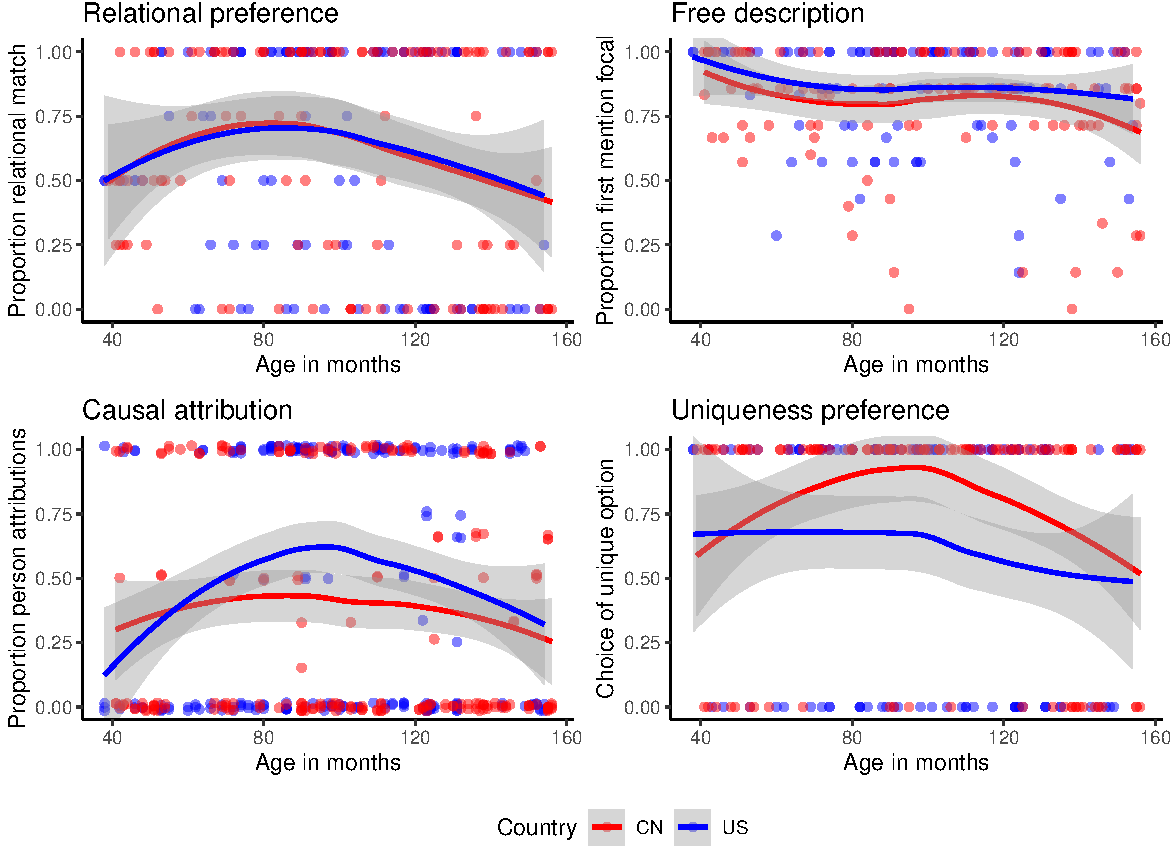
\includegraphics[width=1\linewidth]{figs/mega_fig-1} 

}

\caption[Developmental trajectories in all four tasks]{Developmental trajectories in all four tasks. Each dot summarizes data from one child in our cross-sectional sample between 3 and 12 years, with age in months plotted along the x-axis. Children from the CN sample are shown in red and those from the US in blue, with LOESS fit lines colored accordingly.}\label{fig:mega_fig}
\end{figure*}
\end{CodeChunk}

\hypertarget{results}{%
\section{Results}\label{results}}

We pre-registered the sample size and analyses, available at
\url{https://aspredicted.org/gy8k4.pdf}. All data and analysis scripts
are available at {[}blinded for review{]}. We diverged from analyses
used in previous studies to follow a standardized analysis approach,
fitting mixed effects models with maximal random effect structure for
each task (Barr, Levy, Scheepers, \& Tily, 2013). We adhered to our lab
standard protocol of pruning random slopes and then random intercepts if
a model failed to converge.

Results from all tasks are shown in Figure 2, and we review findings
from each below.

\hypertarget{relational-preference}{%
\subsection{Relational Preference}\label{relational-preference}}

To examine whether children from the two countries show differing
preferences for object- or relation-based reasoning, we used a logistic
mixed effect model to predict response choice with country (CN/US), age
(in months, and scaled), and their interaction as fixed effects. We did
not find an effect of age or country on response bias (US: \emph{M} =
0.38; CN: \emph{M} = 0.41). Following our preregistration, we also fit a
model to predict first trial choice with culture, age (months, scaled),
and their interaction as fixed effects, but did not find any effects
(US: M = 0.34; CN: M = 0.33).

\hypertarget{picture-free-description-1}{%
\subsection{Picture Free Description}\label{picture-free-description-1}}

This task investigated whether children from the US and China differ in
their visual attention, which is reflected in the content of their
description. Following Imada et al.~(2013), we coded whether the first
item children mentioned was the focal object or part of the background.
We predicted this first mentioned item (focal or background) with a
mixed-effect logistic regression model using cultural context, age
(months, scaled), and their interaction as fixed effects. Random
intercepts for each subject and trial number were also included in the
model, as well as random slopes by-trial for cultural context. This
model failed to converge and we pruned the by-trial random slopes. There
was a main effect of country in the predicted direction, with US
children producing more focal first mentions (US: \emph{M} = 0.86; CN:
\emph{M} = 0.81; \(\beta =\) 0.55, z = 2.06, p = 0.04). For the full
description, we ran a Poisson regression model to predict the number of
references children made to any part of the scene per trial with
interaction between description type (focal/background), cultural
context (CN/US), and age (months, scaled) as fixed effects, subject and
trial number as random effects, by-subject random slopes for description
type and by-trial random slopes for cultural context. This model did not
converge either, and we pruned the by-trial random slopes. All of the
main effects and two-way interactions were significant, with effects
resembling that in the first mention analysis (all \emph{p} \textless{}
.05).

\hypertarget{causal-attribution-1}{%
\subsection{Causal Attribution}\label{causal-attribution-1}}

To examine whether Chinese and US children differ in their tendency to
make situational or personal attributions, we ran a mixed-effects
Poisson regression predicting number of situational attributions with
cultural context, age (months, scaled), and their interaction as fixed
effects, subject and trial number as random effects, and random slopes
by-trial for culture. This model did not converge. Following standard
procedure, we iteratively pruned the model to only include the fixed
effect of cultural context, age, and their interaction, and the
intercept of subject. We found main effects of both country (US:
\emph{M} = 0.58; CN: \emph{M} = 0.82; \(\beta =\) -0.32, z = -2.37, p =
0.02) and age (\(\beta =\) 0.18, z = 2.19, p = 0.03). Consistent with
our prediction, we found that US children tended to make fewer situation
attributions than their peers in China, though situational attributions
increased with age in both cultural contexts.

\hypertarget{uniqueness-preference-1}{%
\subsection{Uniqueness Preference}\label{uniqueness-preference-1}}

For this task, we asked whether children from China and the US exhibit
varying preferences for uniqueness or harmony. We ran a simple logistic
regression predicting participants' choice (unique vs.~non-unique
sticker) with cultural context (US or China), age (months, scaled), and
their interaction as fixed effects. We found a significant effect of
cultural context such that Chinese participants were more likely to
choose the unique sticker (US: \emph{M} = 0.61; CN: \emph{M} = 0.76;
\(\beta =\) -0.72, z = -2.42, p = 0.02). This finding contradicts both
previous findings with a related paradigm in which US adults were more
likely to choose the unique object (Kim \& Markus, 1999) and our own
finding in an identical task with adults, where we observed no
difference by country.

\hypertarget{discussion}{%
\section{Discussion}\label{discussion}}

Outward differences between cultures are very salient, with Western and
East Asian cultures as a prominent comparison pair. The cognitive
underpinnings of these differences have been extensively studied, with
an increasing focus on the developmental origins of cultural
differences. As an attempt to synthesize this literature, here we
conducted replications -- with varying degrees of fidelity to the
original -- of four prominent findings regarding US-China differences in
social and cognitive development. Overall we found evidence for cultural
differences in three of these (picture free description, causal
attribution, and uniqueness preference), though one effect (uniqueness)
went in the opposite of the predicted direction.

Previous work has documented a marked cross-cultural difference in
preferences for object-based or relational solutions in the relational
reasoning task we used (the ambiguous cRMTS paradigm) between 3.0 and
4.0 years of age: preschoolers in the US preferred object-based
solutions and those in China preferring relational solutions (Carstensen
et al., 2019). By adulthood, participants in both countries select at
chance between these options, showing no evidence of a relational bias,
perhaps reflecting awareness of the ambiguous training data (Carstensen
\& Cao et al., 2021, in press). Here, we sought to document the
transition from differently biased preschoolers to similar adult
performance across the two countries, alongside three other tasks that
show cross-cultural variation in skills implicated in relational
reasoning (e.g., Christie et al., 2020). Our data suggests that this
convergence happens quickly: we did not see cross-cultural differences
between the youngest children in our samples. However, representation
within our cross-sectional convenience sample is especially sparse below
age 4 (i.e.~7 US children, 12 CN children), limiting our ability to
detect differences at this age. Intriguingly, the developmental pattern
we observe shows similar, increasing preferences for relational
solutions in both groups until about 9 years of age, and then a fall
back towards the adult pattern with no bias.

The other three tasks showed cross-cultural differences that varied in
their emergence and progression. In the free description task, we
observed a general preference for focal first mentions: children from
both countries tended to start their descriptions by referencing the
focal object throughout early and middle childhood, but this tendency
was stronger among the US children. Although we see a consistent
cross-cultural difference in this task, the magnitude of the effect
never approaches that of adults in Cao \& Carstensen et al (in press),
where 90\% of first mentions were focal among US adults but CN adults
showed a flat distribution with roughly equal likelihood of mentioning
the focal object or the background (Standardized mean differences
between culture: Adults: 1.57; Children: 0.37). Our finding indicates a
continuity in this preference over development in early and middle
childhood, but also suggests that the cultural difference becomes more
pronounced and reliable with age. This gradual development likely
reflects the increasing influence of culturally specific practices that
reinforce different psychological tendencies as children grow.

In both of our social reasoning tasks, causal attribution and uniqueness
preference, cross-cultural differences are most evident in the middle of
our cross-sectional sample. In the causal attribution task, these
differences peak between 8 and 9 years, when US children made the most
personal attributions. This trajectory in US participants is similar to
that observed in Gopnik et al. (2017), who showed a consistent level of
situation attributions across ages when the task suggested personal
causes, but a varying trajectory in the condition suggestive of
situational causes. Specifically, they showed that the youngest and
oldest children in their sample were most sensitive to situational
information, with 4-year-olds and 12--14-year-olds providing more
situational attributions than children in the interceding years and
adults. They explained this U-shaped development by suggesting that
young children are the most data-driven learners, with weaker prior
biases because of their limited experience. With time and exposure to
cultural practices, children in the US gradually develop and strengthen
a bias toward personal explanations for behavior. However, as they
approach adolescence, an important period for social learning, children
become more sensitive to social information in particular, responding
once again like the more data-driven 4-year-olds in a way that is
consistent with the situational evidence in the task. In contrast,
Chinese children in our study show a consistent level of situational
attributions throughout -- much like US children in the person bias
condition of Gopnik et al (ibid). Taken together, these findings suggest
that culturally-specific learning environments may interact with
age-related changes in cognitive flexibility to shape the developmental
trajectory of social reasoning about causation.

As in causal attribution, the cultural differences in our uniqueness
preference task peaked between about 8 and 9 years of age, but with an
effect in the opposite of the predicted direction: while all children
showed a general preference to choose the unique sticker well above
chance, Chinese children did so to a greater extent than those in the
US. One possible explanation for this surprising finding is that
children may have construed our task as one of cooperation. To
accommodate young children, experimenters controlled the cursor during
the experiment, so children were encouraged to select a sticker and keep
it in mind while the experimenter ``guessed'' which sticker they had
chosen, mousing over the randomized array from left to right. Because
there were four identical stickers and one unique sticker, some children
may have realized that choosing the unique sticker would be the most
cooperative action since it would be the easiest to communicate about,
cutting short the guessing game. Indeed, many of the school-age
children, and especially those from China, volunteered that they had
chosen the unique sticker (e.g., ``The yellow one!'') before or during
the guessing phase. Accordingly, performance in this task may not
reflect preferences for unique or harmonious choices, but rather
children's interest in responding cooperatively -- and awareness of the
opportunity to do so -- by choosing something that is easy to talk
about. The cultural differences we observed in this task could therefore
be indicative of cultural norms influencing children's behavior in
cooperative settings, which is consistent with previous findings showing
that children growing up in collectivistic cultural contexts are more
attuned to others' goals and motivated to offer help (Guzman, Do, \&
Kok, 2014; Stewart \& McBride-Chang, 2000).

In summary, the emergence of cross-cultural differences follows a unique
trajectory in each of these tasks. We did not observe cross-cultural
differences in relational bias at any point in our cross-sectional
sample, though we did document a commonality in the initial drift
towards a relational preference and then back toward adult performance,
with no bias in either country. In visual attention, we observed
gradual, increasing differences between 3 and 12 years. In contrast, the
two social reasoning tasks showed the most pronounced differences near
the middle of our cross-sectional sample. Specifically, in causal
attribution, there was a divergence in performance that peaks between 8
and 9 years, while choices in our uniqueness preference task showed more
gradual change and the largest differences during elementary years.

Our task selection was guided by an interest in the cognitive mechanisms
underpinning behavioral differences across cultures and the proximal
environmental contexts that shape the use of these mechanisms. Further
work is needed to identify these mechanisms and their sources, but
across our tasks, we observe the earliest differences within visual
attention, lending preliminary support to the view that cross-cultural
differences in the visual domain may play a role in scaffolding later
variation in social cognition (see, e.g., Masuda \& Nisbett, 2001).

This study followed prior work, and accordingly shared some of the
limitations in the work. We had a relatively large sample of children
compared with other developmental research in this literature, but --
given our broad age range -- our estimates for any particular age group
lack precision. In addition, many of the tasks we replicated had only
one or a small number of trials, further limiting precision of
measurement for individuals, and limiting the maximum correlation
between tasks that could be found. Finally, our sampling process treated
the US and China as relatively monolithic cultures, while in fact there
is substantial within-culture variation in both countries.

These findings highlight the importance of measurement for understanding
cross-cultural differences over development. Each task in our study has
a developmental trajectory of its own, and cultural comparisons must
progress from an understanding of that dynamic process, rather than a
snapshot of static differences. This point is especially important
because sample variation both within and across cultures inevitably
confounds measurement, compounding uncertainty about true differences
between populations. Researchers must first establish that a task is
stable by age, gender, and other sociodemographic factors before it is
possible to make inferences about an observed difference.

This work provides a broad survey of performance across cultural
contexts and childhood development, but further work is needed to
address individual differences (within and between tasks and domains of
cognition more broadly) and longitudinal change in individuals.
Nonetheless, by documenting population-level variation over development,
this study can inform identification of the mechanisms (shared or
unique) that underlie variation and change in reasoning, visual
attention, and social cognition over time and across contexts. We hope
that consistent, larger scale developmental work of the kind we present
here can provide steps toward a robust foundation for cross-cultural
developmental science.

\hypertarget{acknowledgements}{%
\section{Acknowledgements}\label{acknowledgements}}

We would like to acknowledge Toshie Imada for kindly sharing materials,
and the Language and Cognition Lab and Culture Collab group at Stanford
University for helpful feedback on early versions of this work. This
study was funded in part by awards from the McDonnell Foundation and the
Center for the Study of Language and Information at Stanford University
supporting A. Carstensen, and an NSF CAREER Award to C. Walker.

\hypertarget{references}{%
\section{References}\label{references}}

\setlength{\parindent}{-0.1in} 
\setlength{\leftskip}{0.125in}

\noindent

\hypertarget{refs}{}
\begin{CSLReferences}{1}{0}
\leavevmode\vadjust pre{\hypertarget{ref-barr2013random}{}}%
Barr, D. J., Levy, R., Scheepers, C., \& Tily, H. J. (2013). Random
effects structure for confirmatory hypothesis testing: Keep it maximal.
\emph{Journal of Memory and Language}, \emph{68}(3), 255--278.

\leavevmode\vadjust pre{\hypertarget{ref-boucher2011dialectical}{}}%
Boucher, H. C. (2011). The dialectical self-concept II: Cross-role and
within-role consistency, well-being, self-certainty, and authenticity.
\emph{Journal of Cross-Cultural Psychology}, \emph{42}(7), 1251--1271.

\leavevmode\vadjust pre{\hypertarget{ref-cao2021investigating}{}}%
Cao, A., Carstensen, A., Gao, S., \& Frank, M. C. (in press). US-china
differences in cognition and perception across 12 tasks: Replicability,
robustness, and within-culture variation. In \emph{Journal of
experimental psychology: general}.

\leavevmode\vadjust pre{\hypertarget{ref-carstensen2021investigating}{}}%
Carstensen, A., Cao, A., Gao, S., \& Frank, M. C. (2021). Investigating
cross-cultural differences in reasoning, vision, and social cognition
through replication. In \emph{Proceedings of the annual meeting of the
cognitive science society} (Vol. 43).

\leavevmode\vadjust pre{\hypertarget{ref-carstensen2019context}{}}%
Carstensen, A., Zhang, J., Heyman, G. D., Fu, G., Lee, K., \& Walker, C.
M. (2019). Context shapes early diversity in abstract thought.
\emph{Proceedings of the National Academy of Sciences}, \emph{116}(28),
13891--13896.

\leavevmode\vadjust pre{\hypertarget{ref-ChalnickBillman1988a}{}}%
Chalnick, A., \& Billman, D. (1988). Unsupervised learning of
correlational structure. In \emph{Proceedings of the tenth annual
conference of the cognitive science society} (pp. 510--516). Hillsdale,
NJ: Lawrence Erlbaum Associates.

\leavevmode\vadjust pre{\hypertarget{ref-chan2011english}{}}%
Chan, C. C. Y., Tardif, T., Chen, J., Pulverman, R. B., Zhu, L., \&
Meng, X. (2011). English-and chinese-learning infants map novel labels
to objects and actions differently. \emph{Developmental Psychology},
\emph{47}(5), 1459--1471.

\leavevmode\vadjust pre{\hypertarget{ref-cheng2020development}{}}%
Cheng, L. (2020). \emph{The development of cognitive styles among
american and chinese children} (PhD thesis). Harvard University.

\leavevmode\vadjust pre{\hypertarget{ref-christie2020development}{}}%
Christie, S., Gao, Y., \& Ma, Q. (2020). Development of analogical
reasoning: A novel perspective from cross-cultural studies. \emph{Child
Development Perspectives}, \emph{14}(3), 164--170.

\leavevmode\vadjust pre{\hypertarget{ref-chua2005cultural}{}}%
Chua, H. F., Boland, J. E., \& Nisbett, R. E. (2005). Cultural variation
in eye movements during scene perception. \emph{Proceedings of the
National Academy of Sciences}, \emph{102}(35), 12629--12633.

\leavevmode\vadjust pre{\hypertarget{ref-open2015estimating}{}}%
Collaboration, O. S. (2015). Estimating the reproducibility of
psychological science. \emph{Science}, \emph{349}(6251), aac4716.

\leavevmode\vadjust pre{\hypertarget{ref-corriveau2017cultural}{}}%
Corriveau, K. H., DiYanni, C. J., Clegg, J. M., Min, G., Chin, J., \&
Nasrini, J. (2017). Cultural differences in the imitation and
transmission of inefficient actions. \emph{Journal of Experimental Child
Psychology}, \emph{161}, 1--18.

\leavevmode\vadjust pre{\hypertarget{ref-decasper1980human}{}}%
DeCasper, A. J., \& Fifer, W. P. (1980). Of human bonding: Newborns
prefer their mothers' voices. \emph{Science}, \emph{208}(4448),
1174--1176.

\leavevmode\vadjust pre{\hypertarget{ref-diyanni2015role}{}}%
DiYanni, C. J., Corriveau, K. H., Kurkul, K., Nasrini, J., \& Nini, D.
(2015). The role of consensus and culture in children's imitation of
inefficient actions. \emph{Journal of Experimental Child Psychology},
\emph{137}, 99--110.

\leavevmode\vadjust pre{\hypertarget{ref-Feigenbaum1963a}{}}%
Feigenbaum, E. A. (1963). The simulation of verbal learning behavior. In
E. A. Feigenbaum \& J. Feldman (Eds.), \emph{Computers and thought}. New
York: McGraw-Hill.

\leavevmode\vadjust pre{\hypertarget{ref-frank2017collaborative}{}}%
Frank, M. C., Bergelson, E., Bergmann, C., Cristia, A., Floccia, C.,
Gervain, J., et al.others. (2017). A collaborative approach to infant
research: Promoting reproducibility, best practices, and
theory-building. \emph{Infancy}, \emph{22}(4), 421--435.

\leavevmode\vadjust pre{\hypertarget{ref-Garnier2007}{}}%
Garnier, S., Gautrais, J., \& Theraulaz, G. (2007). {The biological
principles of swarm intelligence}. \emph{Swarm Intelligence},
\emph{1}(1), 3--31.
http://doi.org/\href{https://doi.org/10.1007/s11721-007-0004-y}{10.1007/s11721-007-0004-y}

\leavevmode\vadjust pre{\hypertarget{ref-gennetian2022open}{}}%
Gennetian, L. A., Frank, M. C., \& Tamis-LeMonda, C. S. (2022). Open
science in developmental science. \emph{Annual Review of Developmental
Psychology}, \emph{4}, 377--397.

\leavevmode\vadjust pre{\hypertarget{ref-gopnik2017changes}{}}%
Gopnik, A., O'Grady, S., Lucas, C. G., Griffiths, T. L., Wente, A.,
Bridgers, S., \ldots{} Dahl, R. E. (2017). Changes in cognitive
flexibility and hypothesis search across human life history from
childhood to adolescence to adulthood. \emph{Proceedings of the National
Academy of Sciences}, \emph{114}(30), 7892--7899.

\leavevmode\vadjust pre{\hypertarget{ref-de2014cultural}{}}%
Guzman, M. R. T. de, Do, K.-A., \& Kok, C. M. (2014). The cultural
contexts of children's prosocial behaviors. \emph{Prosocial Development:
A Multidimensional Approach}, \emph{1}, 221--241.

\leavevmode\vadjust pre{\hypertarget{ref-Hill1983a}{}}%
Hill, J. A. C. (1983). A computational model of language acquisition in
the two-year old. \emph{Cognition and Brain Theory}, \emph{6}, 287--317.

\leavevmode\vadjust pre{\hypertarget{ref-imada2013east}{}}%
Imada, T., Carlson, S. M., \& Itakura, S. (2013). East--west cultural
differences in context-sensitivity are evident in early childhood.
\emph{Developmental Science}, \emph{16}(2), 198--208.

\leavevmode\vadjust pre{\hypertarget{ref-ji2001culture}{}}%
Ji, L.-J., Nisbett, R. E., \& Su, Y. (2001). Culture, change, and
prediction. \emph{Psychological Science}, \emph{12}(6), 450--456.

\leavevmode\vadjust pre{\hypertarget{ref-ji2000culture}{}}%
Ji, L.-J., Peng, K., \& Nisbett, R. E. (2000). Culture, control, and
perception of relationships in the environment. \emph{Journal of
Personality and Social Psychology}, \emph{78}(5), 943--955.

\leavevmode\vadjust pre{\hypertarget{ref-ji2004culture}{}}%
Ji, L.-J., Zhang, Z., \& Nisbett, R. E. (2004). Is it culture or is it
language? Examination of language effects in cross-cultural research on
categorization. \emph{Journal of Personality and Social Psychology},
\emph{87}(1), 57--65.

\leavevmode\vadjust pre{\hypertarget{ref-kim1999deviance}{}}%
Kim, H., \& Markus, H. R. (1999). Deviance or uniqueness, harmony or
conformity? A cultural analysis. \emph{Journal of Personality and Social
Psychology}, \emph{77}(4), 785.

\leavevmode\vadjust pre{\hypertarget{ref-koo2018analytic}{}}%
Koo, M., Choi, J. A., \& Choi, I. (2018). Analytic versus holistic
cognition: Constructs and measurement.

\leavevmode\vadjust pre{\hypertarget{ref-kwan1997pancultural}{}}%
Kwan, V. S. Y., Bond, M. H., \& Singelis, T. M. (1997). Pancultural
explanations for life satisfaction: Adding relationship harmony to
self-esteem. \emph{Journal of Personality and Social Psychology},
\emph{73}(5), 1038--1051.

\leavevmode\vadjust pre{\hypertarget{ref-Lewis1978a}{}}%
Lewis, C. (1978). \emph{Production system models of practice effects}
(Doctoral dissertation). Department of Psychology, University of
Michigan, Ann Arbor.

\leavevmode\vadjust pre{\hypertarget{ref-liang2012effect}{}}%
Liang, B., \& He, Y. (2012). The effect of culture on consumer choice:
The need for conformity vs. The need for uniqueness. \emph{International
Journal of Consumer Studies}, \emph{36}(3), 352--359.

\leavevmode\vadjust pre{\hypertarget{ref-mampe2009newborns}{}}%
Mampe, B., Friederici, A. D., Christophe, A., \& Wermke, K. (2009).
Newborns' cry melody is shaped by their native language. \emph{Current
Biology}, \emph{19}(23), 1994--1997.

\leavevmode\vadjust pre{\hypertarget{ref-markus1991culture}{}}%
Markus, H. R., \& Kitayama, S. (1991). Culture and the self:
Implications for cognition, emotion, and motivation. \emph{Psychological
Review}, \emph{98}(2), 224--253.

\leavevmode\vadjust pre{\hypertarget{ref-markus2010cultures}{}}%
Markus, H. R., \& Kitayama, S. (2010). Cultures and selves: A cycle of
mutual constitution. \emph{Perspectives on Psychological Science},
\emph{5}(4), 420--430.

\leavevmode\vadjust pre{\hypertarget{ref-masuda2001attending}{}}%
Masuda, T., \& Nisbett, R. E. (2001). Attending holistically versus
analytically: Comparing the context sensitivity of japanese and
americans. \emph{Journal of Personality and Social Psychology},
\emph{81}(5), 922.

\leavevmode\vadjust pre{\hypertarget{ref-miyamoto2013culture}{}}%
Miyamoto, Y. (2013). Culture and analytic versus holistic cognition:
Toward multilevel analyses of cultural influences. In \emph{Advances in
experimental social psychology} (Vol. 47, pp. 131--188). Elsevier.

\leavevmode\vadjust pre{\hypertarget{ref-moon1993two}{}}%
Moon, C., Cooper, R. P., \& Fifer, W. P. (1993). Two-day-olds prefer
their native language. \emph{Infant Behavior and Development},
\emph{16}(4), 495--500.

\leavevmode\vadjust pre{\hypertarget{ref-morris1994culture}{}}%
Morris, M. W., \& Peng, K. (1994). Culture and cause: American and
chinese attributions for social and physical events. \emph{Journal of
Personality and Social Psychology}, \emph{67}(6), 949.

\leavevmode\vadjust pre{\hypertarget{ref-muthukrishna2020beyond}{}}%
Muthukrishna, M., Bell, A. V., Henrich, J., Curtin, C. M., Gedranovich,
A., McInerney, J., \& Thue, B. (2020). Beyond western, educated,
industrial, rich, and democratic (WEIRD) psychology: Measuring and
mapping scales of cultural and psychological distance.
\emph{Psychological Science}, \emph{31}(6), 678--701.

\leavevmode\vadjust pre{\hypertarget{ref-na2010cultural}{}}%
Na, J., Grossmann, I., Varnum, M. E. W., Kitayama, S., Gonzalez, R., \&
Nisbett, R. E. (2010). Cultural differences are not always reducible to
individual differences. \emph{Proceedings of the National Academy of
Sciences}, \emph{107}(14), 6192--6197.

\leavevmode\vadjust pre{\hypertarget{ref-NewellSimon1972a}{}}%
Newell, A., \& Simon, H. A. (1972). \emph{Human problem solving}.
Englewood Cliffs, NJ: Prentice-Hall.

\leavevmode\vadjust pre{\hypertarget{ref-OhlssonLangley1985a}{}}%
Ohlsson, S., \& Langley, P. (1985). \emph{Identifying solution paths in
cognitive diagnosis} (No. CMU-RI-TR-85-2). Pittsburgh, PA: Carnegie
Mellon University, The Robotics Institute.

\leavevmode\vadjust pre{\hypertarget{ref-oyserman2002rethinking}{}}%
Oyserman, D., Coon, H. M., \& Kemmelmeier, M. (2002). Rethinking
individualism and collectivism: Evaluation of theoretical assumptions
and meta-analyses. \emph{Psychological Bulletin}, \emph{128}(1), 3--72.

\leavevmode\vadjust pre{\hypertarget{ref-peng1999culture}{}}%
Peng, K., \& Nisbett, R. E. (1999). Culture, dialectics, and reasoning
about contradiction. \emph{American Psychologist}, \emph{54}(9), 741.

\leavevmode\vadjust pre{\hypertarget{ref-richland2010young}{}}%
Richland, L. E., Chan, T.-K., Morrison, R. G., \& Au, T. K.-F. (2010).
Young children's analogical reasoning across cultures: Similarities and
differences. \emph{Journal of Experimental Child Psychology},
\emph{105}(1-2), 146--153.

\leavevmode\vadjust pre{\hypertarget{ref-sabbagh2006development}{}}%
Sabbagh, M. A., Xu, F., Carlson, S. M., Moses, L. J., \& Lee, K. (2006).
The development of executive functioning and theory of mind: A
comparison of chinese and US preschoolers. \emph{Psychological Science},
\emph{17}(1), 74--81.

\leavevmode\vadjust pre{\hypertarget{ref-seiver2013did}{}}%
Seiver, E., Gopnik, A., \& Goodman, N. D. (2013). Did she jump because
she was the big sister or because the trampoline was safe? Causal
inference and the development of social attribution. \emph{Child
Development}, \emph{84}(2), 443--454.

\leavevmode\vadjust pre{\hypertarget{ref-ShragerLangley1990a}{}}%
Shrager, J., \& Langley, P. (Eds.). (1990). \emph{Computational models
of scientific discovery and theory formation}. San Mateo, CA: Morgan
Kaufmann.

\leavevmode\vadjust pre{\hypertarget{ref-singelis1994measurement}{}}%
Singelis, T. M. (1994). The measurement of independent and
interdependent self-construals. \emph{Personality and Social Psychology
Bulletin}, \emph{20}(5), 580--591.

\leavevmode\vadjust pre{\hypertarget{ref-spencer2009dialectical}{}}%
Spencer-Rodgers, J., Boucher, H. C., Mori, S. C., Wang, L., \& Peng, K.
(2009). The dialectical self-concept: Contradiction, change, and holism
in east asian cultures. \emph{Personality and Social Psychology
Bulletin}, \emph{35}(1), 29--44.

\leavevmode\vadjust pre{\hypertarget{ref-spencer2007culture}{}}%
Spencer-Rodgers, J., Williams, M. J., Hamilton, D. L., Peng, K., \&
Wang, L. (2007). Culture and group perception: Dispositional and
stereotypic inferences about novel and national groups. \emph{Journal of
Personality and Social Psychology}, \emph{93}(4), 525--543.

\leavevmode\vadjust pre{\hypertarget{ref-stewart2000influences}{}}%
Stewart, S. M., \& McBride-Chang, C. (2000). Influences on children's
sharing in a multicultural setting. \emph{Journal of Cross-Cultural
Psychology}, \emph{31}(3), 333--348.

\leavevmode\vadjust pre{\hypertarget{ref-takemura2007two}{}}%
Takemura, K., Yuki, M., Maddux, W., \& Ohtsubo, Y. (2007). Two types of
collectivism: Intragroup relationship orientation in japan and
intergroup comparison orientation in the united states. \emph{INSEAD
Business School Research Paper}, (2007/54).

\leavevmode\vadjust pre{\hypertarget{ref-tan2020chinese}{}}%
Tan, B. (2020). \emph{Chinese and US young children's executive function
and its sociocultural antecedents}. The University of Memphis.

\leavevmode\vadjust pre{\hypertarget{ref-tardif1996nouns}{}}%
Tardif, T. (1996). Nouns are not always learned before verbs: Evidence
from mandarin speakers' early vocabularies. \emph{Developmental
Psychology}, \emph{32}(3), 492--504.

\leavevmode\vadjust pre{\hypertarget{ref-waxman2016early}{}}%
Waxman, S. R., Fu, X., Ferguson, B., Geraghty, K., Leddon, E., Liang,
J., \& Zhao, M.-F. (2016). How early is infants' attention to objects
and actions shaped by culture? New evidence from 24-month-olds raised in
the US and china. \emph{Frontiers in Psychology}, \emph{7}, 97--107.

\leavevmode\vadjust pre{\hypertarget{ref-wong2018emperor}{}}%
Wong, Y. J., Wang, S.-Y., \& Klann, E. M. (2018). The emperor with no
clothes: A critique of collectivism and individualism. \emph{Archives of
Scientific Psychology}, \emph{6}(1), 251--260.

\end{CSLReferences}

\bibliographystyle{apacite}


\end{document}
